\section{Theorie}
\label{sec:theorie}

    In diesem Abschnitt sollen die theoretischen Grundlagen eines Lock-In-Verstärkers erläutert
    werden.\\
    \\
    Ein Lock-In-Verstärker dient dazu, 
    stark verrauschte Signal zu messen.
    Das Signal wird dabei entrauscht und zusätzlich noch verstärkt. 
    Zu diesem Zweck enthält er einen integrierten phasenempfindlichen Detektor. 
    Der grundsätzliche Aufbau eines Lock-In-Verstärker ist in der folgenden Abbildung 1 dargestellt.
    \begin{figure}[H]
        \centering
        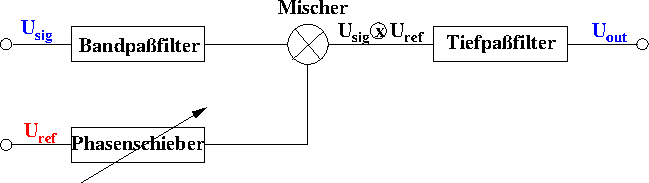
\includegraphics[scale=1]{content/img/Abb_1.pdf}
        \caption{Der grundlegende Aufbau eines Lock-In-Verstärkers.}
        \label{fig:grundaufbau}
    \end{figure}
    Um das Eingangssignal $U_\text{Sig}$ zu entrauschen, 
    wird eine Modulation mit einer Referenzfrequenz $\omega_0$ durchgeführt.\\
    Mithilfe eines Bandpassfilters werden hohe Frequenzen $\omega \gg \omega_0$ und niedrige Frequenzen $\omega \ll \omega_0$ aus dem Eingangssignal herausgefiltert. 
    Der Phasenverschieber dient dazu, 
    die Phasenlage $\phi$ der Referenzfrequenz zu verändern, 
    wobei diese bei $\symup{\Delta}\phi = 0$ mit dem Signal synchronisiert werden kann. 
    Es ensteht eine Referenzspannung $U_\text{Ref}$ mit der Referenzfrequenz $\omega_0$,
    welche in einem Mischer mit dem Eingangssignal multipliziert wird,
    wodurch das Mischsignal $U_\text{Sig} \times U_\text{Ref}$ entsteht. 
    Anschließend wird das Mischsignal in einem Tiefpass ($\tau = RC \gg \frac{1}{\omega_0}$) über mehrere Perioden von $\omega_0$ integriert, 
    was dazu führt, dass die Frequenzbeiträge, 
    welche nicht mit der Referenzfrequenz synchronisiert sind, 
    herausgemittelt werden. 
    Das Ausgangssignal ist eine Gleichspannung $U_\text{Out}$, welche
    proportional zur Eingangsspannung $U_\text{Sig}$ ist und mit
    \begin{equation*}
        U_\text{Out} = U_0 \cos{(\phi)}
    \end{equation*}
    beschrieben werden kann. 
    Mithilfe des Tiefpasses kann zusätzlich die Bandbreite des Restrauschens kontrolliert werden. 
    Bei einer hoher Zeitkonstante $\tau = RC$ können kleine Bandbreiten und somit hohe Güten von $𝑄 = 100\,000$ erreicht werden.\\
    \\
    Im Folgenden soll nun beispielhaft eine sinusförmige Signalspannung betrachtet werden
    \begin{equation*}
        U_\text{Sig} = U_0 \sin{(\omega t)} .
    \end{equation*}
    Die Referenzfrequenz $U_\text{Ref}$ hat die Form einer Rechteckspannung und die gleiche Frequenz.
    \begin{figure}[H]
        \centering
        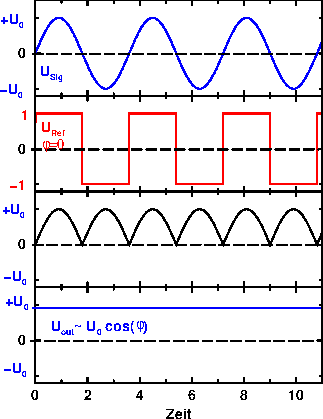
\includegraphics[scale=0.9]{content/img/Abb_2.pdf}
        \caption{Der zeitliche Verlauf der Signal-, der Referenz-, der Misch- und der Ausgangsspannung.}
        \label{fig:signalverläufe}
    \end{figure}
    Die Abbildung \ref{fig:signalverläufe} zeigt die Verläufe der sinusförmigen Signalspannung und der Referenzspannung,
    welche einen Schalter oder Chopper darstellt.
    %Bei einer positiven Amplitude,
    %welche auf $1$ normiert ist,
    %ist der Schalter geöffnet und bei einer negativen Amplitude ist er geschlossen.
    Die Referenzspannung kann durch eine Fourierreihe genähert werden 
    \begin{equation*}
        U_\text{Ref} = \frac{4}{\symup{\pi}} \Bigl(\sin{(\omega t)} + \frac{1}{3}\sin{(3\omega t)} + \frac{1}{5}\sin{(5\omega t)} + ... \Bigr) .
    \end{equation*}
    Für die Mischspannung ergibt sich danach
    \begin{equation*}
        U_\text{Sig} \times U_\text{Ref} = \frac{2}{\symup{\pi}} U_0 \Bigl(1 - \frac{2}{3}\cos{(2\omega t)} - \frac{2}{15}\cos{(4\omega t)} - \frac{2}{35}\cos{(6\omega t)} + ... \Bigr) ,
    \end{equation*}
    sie besteht also aus den geraden Oberwellen der Frequenz $\omega$.
    Der Tiefpass sorgt anschließend dafür,
    dass diese Oberwellen unterdrückt werden.
    Für $\phi = 0$ ergibt sich damit die maximale Ausgangsspannung 
    \begin{equation*}
        U_\text{Out} = \frac{2}{\symup{\pi}} U_0 ,
    \end{equation*}
    welche wieder eine Gleichspannung und proportional zur Signalspannung $U_\text{Sig}$ ist.
    Für eine feste Phasendifferenz $\phi \neq 0$ ergibt sich die Ausgangsspannung
    \begin{equation}
        U_\text{Out} = \frac{2}{\symup{\pi}} U_0 \cos{\phi} ,
        \label{eqn:ausgangsspannung_phase}
    \end{equation}
    welche demnach abhängig von der Phasendifferenz $\phi$ ist.
    